% Chapter Template

\chapter{Bilan} % Main chapter title

\label{Chapter4} % Change X to a consecutive number; for referencing this chapter elsewhere, use \ref{ChapterX}

\lhead{Chapter X. \emph{Chapter Title Here}} % Change X to a consecutive number; this is for the header on each page - perhaps a shortened title

%----------------------------------------------------------------------------------------
%	SECTION 1
%----------------------------------------------------------------------------------------

\section{Planning Effectif}

%-----------------------------------
%	SUBSECTION 1
%-----------------------------------
\subsection{Planning horaire}

\begin{table}[h]
\centering
\resizebox{\textwidth}{!}{%
\begin{tabular}{|l|l|l|l|ll}
\cline{1-4}
\multicolumn{1}{|c|}{\textbf{Membres}} & \multicolumn{1}{c|}{\textbf{Séance 1 (17/10--21/10)}}                                                           & \multicolumn{1}{c|}{\textbf{\begin{tabular}[c]{@{}c@{}}Séance 2 \\ (21/10--24/10)\end{tabular}}}                          & \multicolumn{1}{c|}{\textbf{\begin{tabular}[c]{@{}c@{}}Séance 3\\ (24/10--04/11)\end{tabular}}}                                        &  &  \\ \cline{1-4}
Quentin Dupont                         & \begin{tabular}[c]{@{}l@{}}-Description des CU (3h)\\ -Diagramme des CU (1h)\\ -Glossaire (1h)\end{tabular}     & -Description détaillée des CU (4h)                                                                                        & \begin{tabular}[c]{@{}l@{}}-Diagramme de séquences chargement XML (3h)\\ -Parseur du plan (1h)\end{tabular}                            &  &  \\ \cline{1-4}
Salma El Alaoui                        & \begin{tabular}[c]{@{}l@{}}-Planning prévisionnel (2h)\\ -Modèle du domaine (1h)\\ -Glossaire (1h)\end{tabular} & \begin{tabular}[c]{@{}l@{}}-Modèle du domaine (3h)\\ -Diagramme de classes (1h)\end{tabular}                              & \begin{tabular}[c]{@{}l@{}}-Fin du diagramme de classes (3h)\\ -Etude de Choco (1h)\end{tabular}                                       &  &  \\ \cline{1-4}
Donovan Fournier                       & \begin{tabular}[c]{@{}l@{}}-Modèle du domaine (3h)\\ -Glossaire (1h)\end{tabular}                               & \begin{tabular}[c]{@{}l@{}}-Modèle du domaine (3h)\\ -Diagramme de classes (1h)\end{tabular}                              & \begin{tabular}[c]{@{}l@{}}-Fin du diagramme de classes (3h)\\ -Etude de Choco (1h)\end{tabular}                                       &  &  \\ \cline{1-4}
Ségolène Minjard                       & \begin{tabular}[c]{@{}l@{}}-Modèle du domaine (2h)\\ -Description des CU (1h)\\ -Glossaire (1h)\end{tabular}    & \begin{tabular}[c]{@{}l@{}}-Description de l'IHM (1h)\\ -Diagramme de classes (1h)\\ -Modèle du domaine (2h)\end{tabular} & \begin{tabular}[c]{@{}l@{}}-Fin du diagramme de classes (3h)\\ -Diagramme de séquence: Ajout d'un point de livraison (1h)\end{tabular} &  &  \\ \cline{1-4}
Benjamin Legrand                       & \begin{tabular}[c]{@{}l@{}}-Modèle du domaine (1h)\\ -Description des CU (3h)\\ -Glossaire(1h)\end{tabular}     & \begin{tabular}[c]{@{}l@{}}-Description des CU (3h)\\ -Diagramme de classes (1h)\end{tabular}                             & \begin{tabular}[c]{@{}l@{}}-Fin du diagramme de classes (3h)\\ -Diagramme de séquence: Ajout d'un point de livraison (1h)\end{tabular} &  &  \\ \cline{1-4}
Zied Thabet                            & \begin{tabular}[c]{@{}l@{}}-Description des CU (1h)\\ -Diagramme des -CU (3h)\\ -Glossaire (1h)\end{tabular}    & \begin{tabular}[c]{@{}l@{}}-Description de l'IHM (1h)\\ -Description détaillée des CU (3h)\end{tabular}                   & \begin{tabular}[c]{@{}l@{}}-Diagramme de séquences chargement XML (3h)\\ -Parseur du plan (1h)\end{tabular}                            &  &  \\ \cline{1-4}
Total                                  & \multicolumn{1}{r|}{\textbf{24h}}                                                                               & \multicolumn{1}{r|}{\textbf{24h}}                                                                                         & \multicolumn{1}{r|}{\textbf{24h}}                                                                                                      &  &  \\ \cline{1-4}
\end{tabular}
}
\caption{Planning horaire-début}
\label{my-label}
\end{table}

% Please add the following required packages to your document preamble:
% \usepackage{graphicx}
\begin{table}[h]
\centering
\resizebox{\textwidth}{!}{%
\begin{tabular}{|l|l|l|}
\hline
\multicolumn{1}{|c|}{\textbf{Membres}} & \multicolumn{1}{c|}{\textbf{\begin{tabular}[c]{@{}c@{}}Séance 3\\ (04/11--07/11)\end{tabular}}} & \multicolumn{1}{c|}{\textbf{\begin{tabular}[c]{@{}c@{}}Séance 4\\ (07/11--14/11)\end{tabular}}} \\ \hline
Quentin Dupont & \begin{tabular}[c]{@{}l@{}}-Parseur de la demande de livraison (3h)\\ -Vérification des diagrammes de séquence (1h)\end{tabular} & \begin{tabular}[c]{@{}l@{}}-Lecture et Validation XML (6h)\\ -Gestion des erreurs et warnings (4h)\\ -Tests (1h)\end{tabular} \\ \hline
Salma El Alaoui & \begin{tabular}[c]{@{}l@{}}-Diagramme de séquences : Calcul d'une tournée (3h)\\ -Génération automatique à partir du diagramme de classes (1h)\end{tabular} & \begin{tabular}[c]{@{}l@{}}-Calcul d'une tournée (6h)\\ -Résolution de bugs (3h)\\ -Rapport LateX (8h)\\ -Planning effectif (4h)\\ -Code Reviews (5h)\end{tabular} \\ \hline
Donovan Fournier & \begin{tabular}[c]{@{}l@{}}-Diagramme de séquences : Calcul d'une tournée (4h)\\ -Mise en place Javadoc (1h)\end{tabular} & \begin{tabular}[c]{@{}l@{}}-Implémentation de Dijsktra (2h)\\ -Code Reviews (8h)\\ -Résolution de bugs (8h)\\ -Tests (1h)\end{tabular} \\ \hline
Ségolène Minjard & -Fin des diagrammes de séquences d'ajout d'u point de livraison.(4h) & \begin{tabular}[c]{@{}l@{}}-Ajout/Suppression d'un point (10h)\\ -Undo/Redo (5h)\\ -Binding Contrôleur/Vue (2h)\\ -Tests (1h)\\ -Résolution Bugs (2h)\\ -Affichage d'informations sur la livraison(1h)\end{tabular} \\ \hline
Benjamin Legrand & \begin{tabular}[c]{@{}l@{}}-Méthodes utiles pour l'IHM (3h)\\ -Vérification des diagrammes de séquence (1h)\end{tabular} & \begin{tabular}[c]{@{}l@{}}-Visualisation du plan + demande livraison (18h)\\ -Détails IHM (4h)\\ -Affichage d'informations sur la livraison (3h)\end{tabular} \\ \hline
Zied Thabet & \begin{tabular}[c]{@{}l@{}}-Parseur de la demande de livraison (2h)\\ -Vérification des diagrammes de séquence (2h)\end{tabular} & \begin{tabular}[c]{@{}l@{}}-Lecture et validation XML (12h)\\ -Binding Modèle/Vue (2h)\\ -Génération fichier txt(4h)\\ -Tests (1h)\end{tabular} \\ \hline
Total & \multicolumn{1}{r|}{\textbf{25h}} & \multicolumn{1}{r|}{\textbf{128h}} \\ \hline
\end{tabular}
}
\caption{Planning horaire-fin}
\label{my-label}
\end{table}

\clearpage
\subsection{Planning Effectif}
\begin{figure}[htbp]
	\centering
		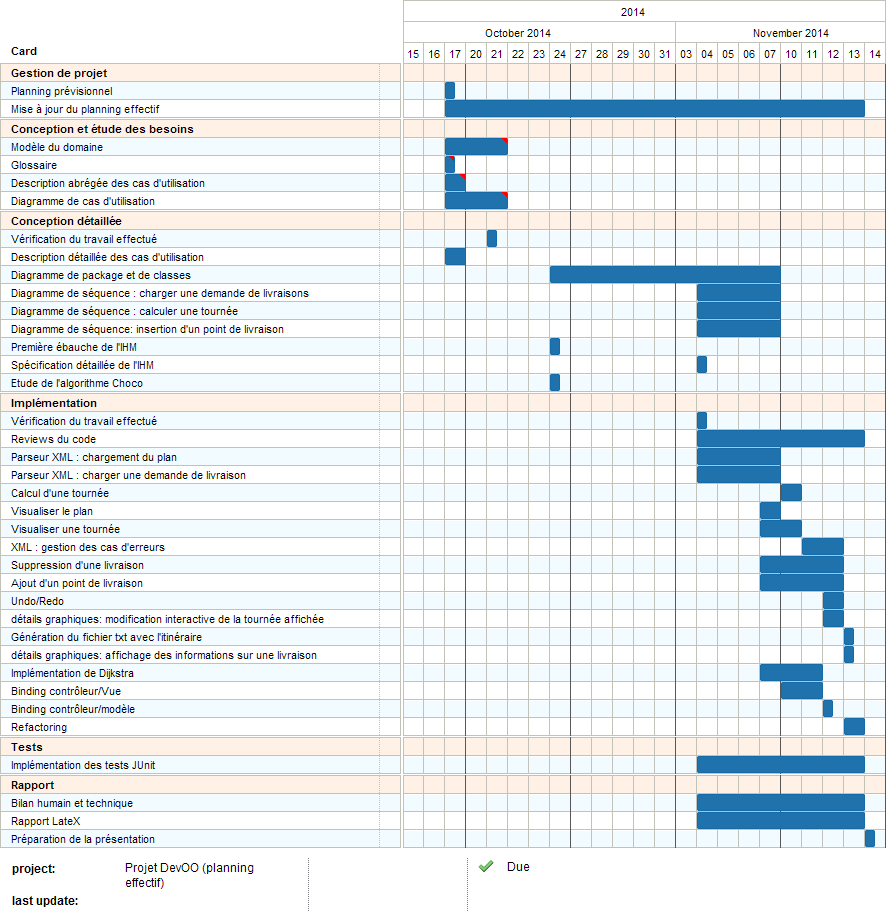
\includegraphics[width=\textwidth,height=\textheight,keepaspectratio]{Figures/effective_plan}
		\rule{35em}{0.5pt}
	\caption[Planning effectif du projet]{Planning effectif du projet}
\end{figure}
\clearpage

%----------------------------------------------------------------------------------------
%	SECTION 2
%----------------------------------------------------------------------------------------

\section{Bilan humain}

Sed ullamcorper quam eu nisl interdum at interdum enim egestas. Aliquam placerat justo sed lectus lobortis ut porta nisl porttitor. Vestibulum mi dolor, lacinia molestie gravida at, tempus vitae ligula. Donec eget quam sapien, in viverra eros. Donec pellentesque justo a massa fringilla non vestibulum metus vestibulum. Vestibulum in orci quis felis tempor lacinia. Vivamus ornare ultrices facilisis. Ut hendrerit volutpat vulputate. Morbi condimentum venenatis augue, id porta ipsum vulputate in. Curabitur luctus tempus justo. Vestibulum risus lectus, adipiscing nec condimentum quis, condimentum nec nisl. Aliquam dictum sagittis velit sed iaculis. Morbi tristique augue sit amet nulla pulvinar id facilisis ligula mollis. Nam elit libero, tincidunt ut aliquam at, molestie in quam. Aenean rhoncus vehicula hendrerit.


\section{Bilan technique}

Sed ullamcorper quam eu nisl interdum at interdum enim egestas. Aliquam placerat justo sed lectus lobortis ut porta nisl porttitor. Vestibulum mi dolor, lacinia molestie gravida at, tempus vitae ligula. Donec eget quam sapien, in viverra eros. Donec pellentesque justo a massa fringilla non vestibulum metus vestibulum. Vestibulum in orci quis felis tempor lacinia. Vivamus ornare ultrices facilisis. Ut hendrerit volutpat vulputate. Morbi condimentum venenatis augue, id porta ipsum vulputate in. Curabitur luctus tempus justo. Vestibulum risus lectus, adipiscing nec condimentum quis, condimentum nec nisl. Aliquam dictum sagittis velit sed iaculis. Morbi tristique augue sit amet nulla pulvinar id facilisis ligula mollis. Nam elit libero, tincidunt ut aliquam at, molestie in quam. Aenean rhoncus vehicula hendrerit.